%%% lorem.tex --- 
%% 
%% Filename: lorem.tex
%% Description: 
%% Author: Ola Leifler
%% Maintainer: 
%% Created: Wed Nov 10 09:59:23 2010 (CET)
%% Version: $Id$
%% Version: 
%% Last-Updated: Wed Nov 10 09:59:47 2010 (CET)
%%           By: Ola Leifler
%%     Update #: 2
%% URL: 
%% Keywords: 
%% Compatibility: 
%% 
%%%%%%%%%%%%%%%%%%%%%%%%%%%%%%%%%%%%%%%%%%%%%%%%%%%%%%%%%%%%%%%%%%%%%%
%% 
%%% Commentary: 
%% 
%% 
%% 
%%%%%%%%%%%%%%%%%%%%%%%%%%%%%%%%%%%%%%%%%%%%%%%%%%%%%%%%%%%%%%%%%%%%%%
%% 
%%% Change log:
%% 
%% 
%% RCS $Log$
%%%%%%%%%%%%%%%%%%%%%%%%%%%%%%%%%%%%%%%%%%%%%%%%%%%%%%%%%%%%%%%%%%%%%%
%% 
%%% Code:

\chapter{Results}
\label{cha:results}

This chapter presents the results. Note that the results are presented
factually, striving for objectivity as far as possible.  The results
shall not be analyzed, discussed or evaluated.  This is left for the
discussion chapter.

In case the method chapter has been divided into subheadings such as
pre-study, implementation and evaluation, the result chapter should
have the same sub-headings. This gives a clear structure and makes the
chapter easier to write.

In case results are presented from a process (e.g. an implementation
process), the main decisions made during the process must be clearly
presented and justified. Normally, alternative attempts, etc, have
already been described in the theory chapter, making it possible to
refer to it as part of the justification.

\section{Systembeskrivning}

Projektgruppen definierade en tydlig design av applikationen innan implementationen påbörjades. Detta var för att försäkra sig om att applikationen skulle bli av hög kvalitet och eventuella designproblem skulle hittas tidigt i projektet. I figur X kan man se en generell överblick av systemet.

\subsection{Systemanatomi}
Under iteration ett producerade projektgruppen en systemanatomi av applikationen som skulle utveckas. Denna producerades utifrån de use-cases och krav kunden hade tillhandahållit.

\begin{figure}[h]
    \centering
    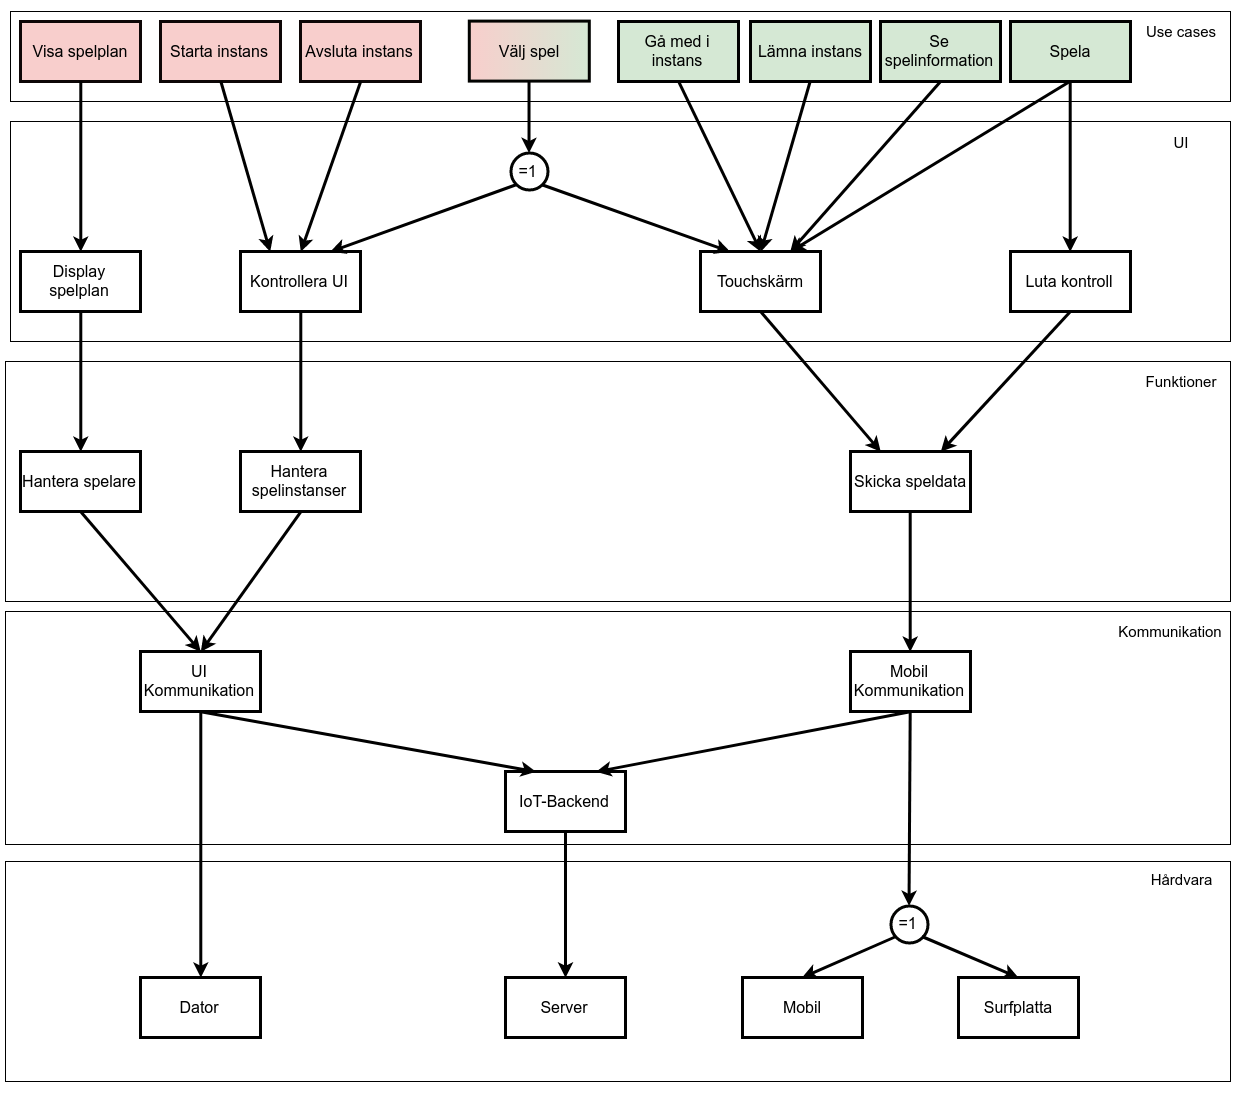
\includegraphics[scale=0.3]{systemanatomi_graf}
    \caption{Överblick av systemanatomin}
    \label{fig:systemanatomi_graf}
\end{figure}

\pagebreak

\subsection{Moduler}
Projektgruppen använde sig av den generella strukturen av systemet, kundens krav och systemanatomin för att skapa en mer detaljerad arkitektur. I figur X kan man se den övergripande strukturen av modulerna som finns i applikationen.

\begin{figure}[h]
    \centering
    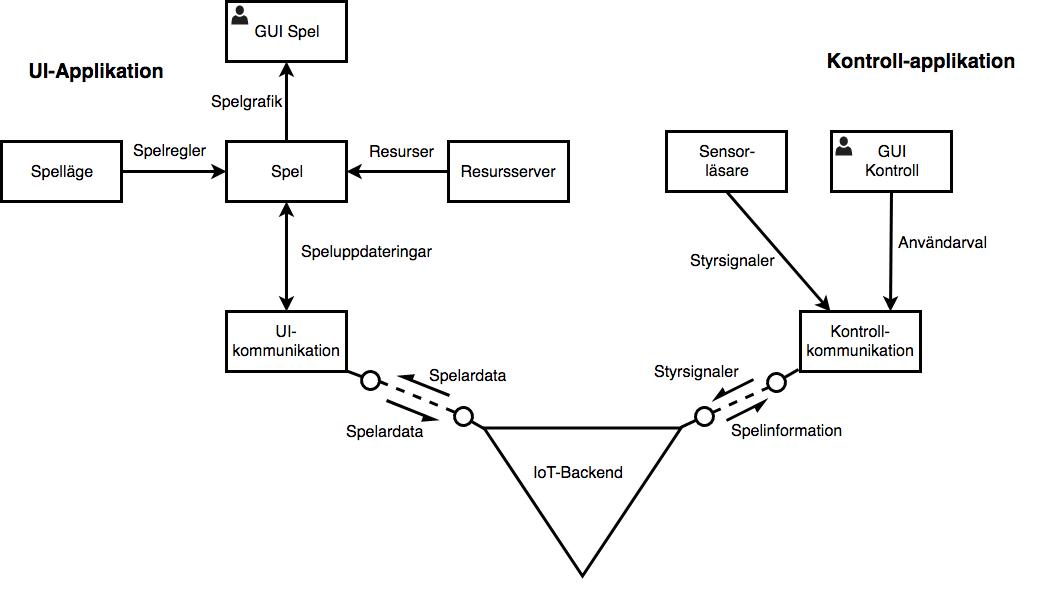
\includegraphics[scale=0.3]{konceptarkitektur}
    \caption{Överblick av systemets moduler}
    \label{fig:konceptarkitektur}
\end{figure}

\pagebreak


\subsubsection*{Ansvarsområden}
Varje modul i systemet har ett eget ansvarsområde. Nedan följer en förtydling på vad varje modul ansvarar för.

\begin{labeling}{\small{\textbf{Kontrollkommunikation}}}
    \item [\small{\textbf{GUI Spel}}]
        \begin{itemize}
            \item Visa upp spelplanen
            \item Visa upp menyer
            \item Starta spel med specifika inställningar
            \newline
        \end{itemize}

    \item [\small{\textbf{Spelläge}}]
        \begin{itemize}
            \item Sätta upp regler för spelet
            \item Avgöra vilka resurser spelet ska innehålla
            \item Avgöra vad som ska ske vid olika tillfällen i spelet
            \newline
        \end{itemize}

    \item [\small{\textbf{Spel}}]
        \begin{itemize}
            \item Hålla koll på de olika spelarna
            \item Tillhandahålla grundläggande spelmekanik
            \newline
        \end{itemize}

    \item [\small{\textbf{Resursserver}}]
        \begin{itemize}
            \item Lagra vilka resurser som finns
            \item Ladda in resurser
            \newline
        \end{itemize}

    \item [\small{\textbf{UI-kommunikation}}]
        \begin{itemize}
            \item Upprätta uppkoppling mot server
            \item Förpacka data för kommunikation
            \newline
        \end{itemize}

    \item [\small{\textbf{Sensorläsare}}]
        \begin{itemize}
            \item Läsa av data från sensor
            \item Abstrahera sensordata till standardiserad form
            \item konfigurera sensor
            \newline
        \end{itemize}

    \item [\small{\textbf{GUI-kontroll}}]
        \begin{itemize}
            \item Visa menyer för att gå med i spelinstans
            \item Visa spelinformation om det pågående spelet
            \item Tillhandahålla knappar på skärmen
            \newline
        \end{itemize}

    \item [\small{\textbf{Kontrollkommunikation}}]
        \begin{itemize}
            \item Upprätta uppkoppling mot server
            \item Förpacka data för kommunikation
            \newline
        \end{itemize}

    \item [\small{\textbf{IoT-Backend}}]
        \begin{itemize}
            \item Dirigera data mellan olika Kontroll-applikationer och olika instanser av UI-applikationen
            \item Verifiera koder för att gå med i specifika spelinstanser
            \newline
        \end{itemize}
\end{labeling}


\section{Gemensamma erfarenheter}
Denna del tar upp diverse erfarenheter projektgruppen råkat ut för, både innan och under projektets gång.


\subsection{Tidigare erfarenheter}
Alla av projektets medlemmar hade studerat mer än två år på respektive program innan detta projekt startades. På grund hade alla haft möjligheten att medverka i några större projekt och var därför ganska vana vid hur arbetet gick till. Dock var det få som hade erfarenhet med webbutveckling och spelprogrammering, något som hade stort fokus i detta projekt. Detta var dock inget större problem då de mer erfarna kunde hjälpa resten att komma igång.

\subsection{Nya erfarenheter}
Under projeketets gång har alla medlemmar fått använda sig av nya verktyg och metoder som de inte haft tidigare erfarenhet av. De projektmedlemmar som tidigare saknade erfarenhet inom webbutveckling och spelprogrammering har fått chansen att sätta sig in i dessa.


\subsection{Tidsbrist}
I början av projektet hade gruppen bra tidsplanering och lämnade in första iterationen i god tid för att sedan ta det lugnt. I början av iteration två satsade gruppen i huvudsak på utveckling och lämnade dokumentskrivning till senare, vilket visade sig vara en missbedömning. Detta ledde till att det blev stressigt framåt slutet av iteration två vilket kan ha påverkat dokumentkvaliteten negativt.

\subsection{Tekniska erfarenheter}
Projektgruppen utvecklade applikationen i ramverket React som har något som kallas för states. Projektgruppen märkte att det snabbt kunde bli något rörigt när man introducerade flera lager av komponenter. Detta problem löser andra webbapplikationer genom extra verktyg för state-hantering, och gruppen reflekterade över dessa men besluta emot att använda något liknande.



%%%%%%%%%%%%%%%%%%%%%%%%%%%%%%%%%%%%%%%%%%%%%%%%%%%%%%%%%%%%%%%%%%%%%%
%%% lorem.tex ends here

%%% Local Variables: 
%%% mode: latex
%%% TeX-master: "demothesis"
%%% End: 
